
\subsection{Pgmpy}
The library to read and represent Bayesian networks is Pgmpy \cite{pgmpy_paper}. With Pgmpy, Bayesian network can be easily created, and it also support reading Bayesian networks from BIF format. The library is opensource so that it can be modified and extended if required. Pgmpy also have build-in inferencing method using Variable Elimination so that the run time can be used to evaluate the performance. 

 \subsection{Extend the Pgmpy library}
    Pgmpy library does not support fetching CPT values using table indexing, the only way to fetch value is through specifying evidence and variables and query the value through Variable Elimination method. The Variable Elimination method is the bayesian inference method that is \textcolor{red}{Insert time complexety}. To solve the problem, I extended the pgmpy library to support fetching variable values without querying using Variable Elimination.\\

    \noindent \textbf{The TabularCPD Class}:\\
    The method get\_cpds returns a conditional probability distribution of the node, the returned type is defined as TabularCPD that contains the name of the node, cardinality, variables which are stores as a nested list, the list of evidences and their corresponding cardinalities. An example is given below:
    \begin{lstlisting}
    cpd = TabularCPD('dysp', 2, [[0.9, 0.7, 0.8, 0.1],
                                 [0.1, 0.3, 0.2, 0.9]],
                                 ['bronc', 'either'], [2, 2])
    \end{lstlisting}

    \noindent \textbf{The storage of a TabularCPD}:\\
    calling cpd.variables() will return a list starts with the node variable followed by the the evidences, and calling cpd.cardinality() will return the cardinality list in the same order as the variables returned by cpd.variables()
    \begin{lstlisting}
    >> print(cpd.variables())
        >> ['dysp', 'bronc', 'either']
    >> print(cpd.cardinality())
        >> ['2', '2', '2']
    \end{lstlisting}

   \noindent \textbf{MyCPD}:\\
    col\_index stores the index of the combination of evidence, in the same order as the probability distribution defined in the \textbf{standard node block}. The col\_index is constructed using the itertools.product in python which return the cartesian product. The transpose of the col\_index correspond to the order of the probability distribution specify in the BIF file. Consider the example with node \textit{dysp}.
    \begin{lstlisting}
    >> col_indexes = np.array(list(product(*[range(i) for i in ev_card])))
    >> print(evidence, col_index) 
        >> ['either', 'bronc']
        >> [[0 0]
            [0 1]
            [1 0]
            [1 1]]
    \end{lstlisting}
   
    \noindent Then the evidences are formatted into tuples with the same length and each column correspond to one entrance to the probability table.\\
    \begin{lstlisting}
    A sample return the evidence entrance. 'dysp' node in aisa.bif
    >> entrance <- [('{s}'.format(s = reverse_ev[i]), d) 
                    for d in col_indexes.T[i]]
        >> [('either',0), ('either',0), ('either',1), ('either',1)]
           [('bronc', 0), ('bronc', 1), ('bronc', 0), ('bronc', 1)]
    Then the entrace are transposed using rol_to_col()
    >> rol_to_col(entrance)
        >> [[('bronc',0), ('either',0)], [('bronc',1), ('either',0)], 
            [('bronc',0), ('either',1)], [('bronc',1), ('either',1)]]
    \end{lstlisting}
    
    \begin{minted}
    [linenos]
    {python}
    Parameter: A TabularCPD
    def myCPD(TabularCPD cpd):
        var, evidence <- cpd.variable[0], cpd.variable[1:]
        var_card, ev_card <- cpd.cardinality[0], cpd.cardinality[1:]
        variable <- [(name, 0),.., (name, n)]
        value = cpd.values()
        # node with evidence:
        if evidence not null:
            col_indexes <- get index
            for i in cardinality:
                entrance <- format the header
                rol_to_col(entrance) # transpose
            for each node variable:
                newcpt.append(variable, index, evidence, corresponding_value)
        # node with no evidence
        else:
            for each node variable
                newcpt.apend(variable, index, [], corresponding_value)
    \end{minted}
    A Sample return of newcpt of node dysp:
    \begin{lstlisting}
    [('dysp', 0, [('bronc', 0), ('either', 0)], 0.9), 
     ('dysp', 0, [('bronc', 1), ('either', 0)], 0.7), 
     ...
     ('dysp', 1, [('bronc', 0), ('either', 1)], 0.2), 
     ('dysp', 1, [('bronc', 1), ('either', 1)], 0.9)]
    \end{lstlisting}
    The method mycpd(TabularCPD) returns a table\-like list of tuples, the first two element in each tuple forms the node variables and the third element is a list of evidence. An example of the first tuple in the list means $dysp_{0}|bronc_{0}either_{0} = 0.9$. Now the returned data support fetching values using list indexing so that we don't need to query the value using the time-consuming Variable Elimination.\\ 
    
    
    \noindent In our case for both bronc and either, the evidence all equals to 2, the convention for the order is shown in figure \ref{fig:sample print table}. The list which store the values are the transpose of the matrix in BIF format.\\
    \begin{figure}
        \centering
        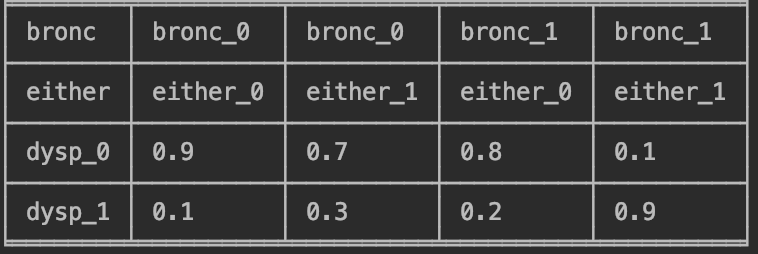
\includegraphics[width = 0.7\textwidth]{pic/printBayesnode.png}
        \caption{A sample printed CPT of a node dyps}
        \label{fig:sample print table}
    \end{figure}
    
\subsection{Storing variables, weights and CNFs}
There are three important storage in the implementation, the generated variables, corresponding weights and the representation of CNFs.\\

\noindent Variables in the CNFs and its corresponding weights are stored in python dictionaries. One of the consideration is the speed of looking up  a certain variable weights or its corresponding integer used in the DIMAC format. Encoding Bayesian networks might lead to dealing with large number of variables. Some of the results \cite{2008-literature-review} shows that the variable numbers might reach over 50,000. \\

\noindent If we use a list of pairs to store the variables or the weights, the time complexity for looking up a list is \textbf{O}(n) for linear search over the list. However, the time complexity for looking up in the dictionary is \textbf{O}(1). When dealing with large number of variables, the time difference is substantial. In addition, adding the dictionary operation 'add' is an process with O(1) regardless of the size of the dictionary. The key in the variable is the name of the variable, \textit{weights} stores its corresponding weight and the var\_dic stores the integer used to represent the variable in the DIMAC format.

\begin{lstlisting}
var_dic = {
    'theta_x1|y1y2': 5,
    ...
}

weights = {
    'theta_x1|y1y2': 0.03,
    ...
}
\end{lstlisting}

\noindent The CNF clauses are stored as a list of lists. Inner list represent one clause that are the disjunction of literals, and the outer list represent the conjunction of the clauses. We use list to store the clauses because once a clause is generated and append to the list, it won't be modified during the later process, and no other operation such as list lookup is needed. The only operation is to traverse each clause in the list that the CNF to write to files.
